\documentclass{article}
\usepackage[a4paper, landscape]{geometry}
\usepackage{tikz}
\usetikzlibrary{shapes.geometric, arrows.meta, positioning}
\usetikzlibrary{positioning, calc, fit}


\tikzstyle{process} = [rectangle, minimum width=3cm, line width = 1.5pt, minimum height=1.5cm, text centered, draw=black, fill=blue!20]

\tikzstyle{process_analysis} = [rectangle, minimum width=3cm, minimum height=1.5cm, text centered, draw=black, fill=blue!10, rounded corners]

\tikzstyle{input} = [rectangle, dashed,rounded corners, minimum width=2cm, minimum height=1.0cm, text centered, draw=black, fill=none]

\tikzstyle{plugin} = [rectangle, rounded corners, minimum width=3cm, minimum height=1.5cm, text centered, draw=black, fill=green!20]

\tikzstyle{arrow_solid} = [thick,->,>=Stealth]

\tikzstyle{arrow_dashed} = [thick,->,>=Stealth, dashed, rounded corners]

% Built using AI assistance from 
% https://www.yeschat.ai/gpts-2OToA4aCXd-TikZ-LaTeX-Expert

\begin{document}
	
	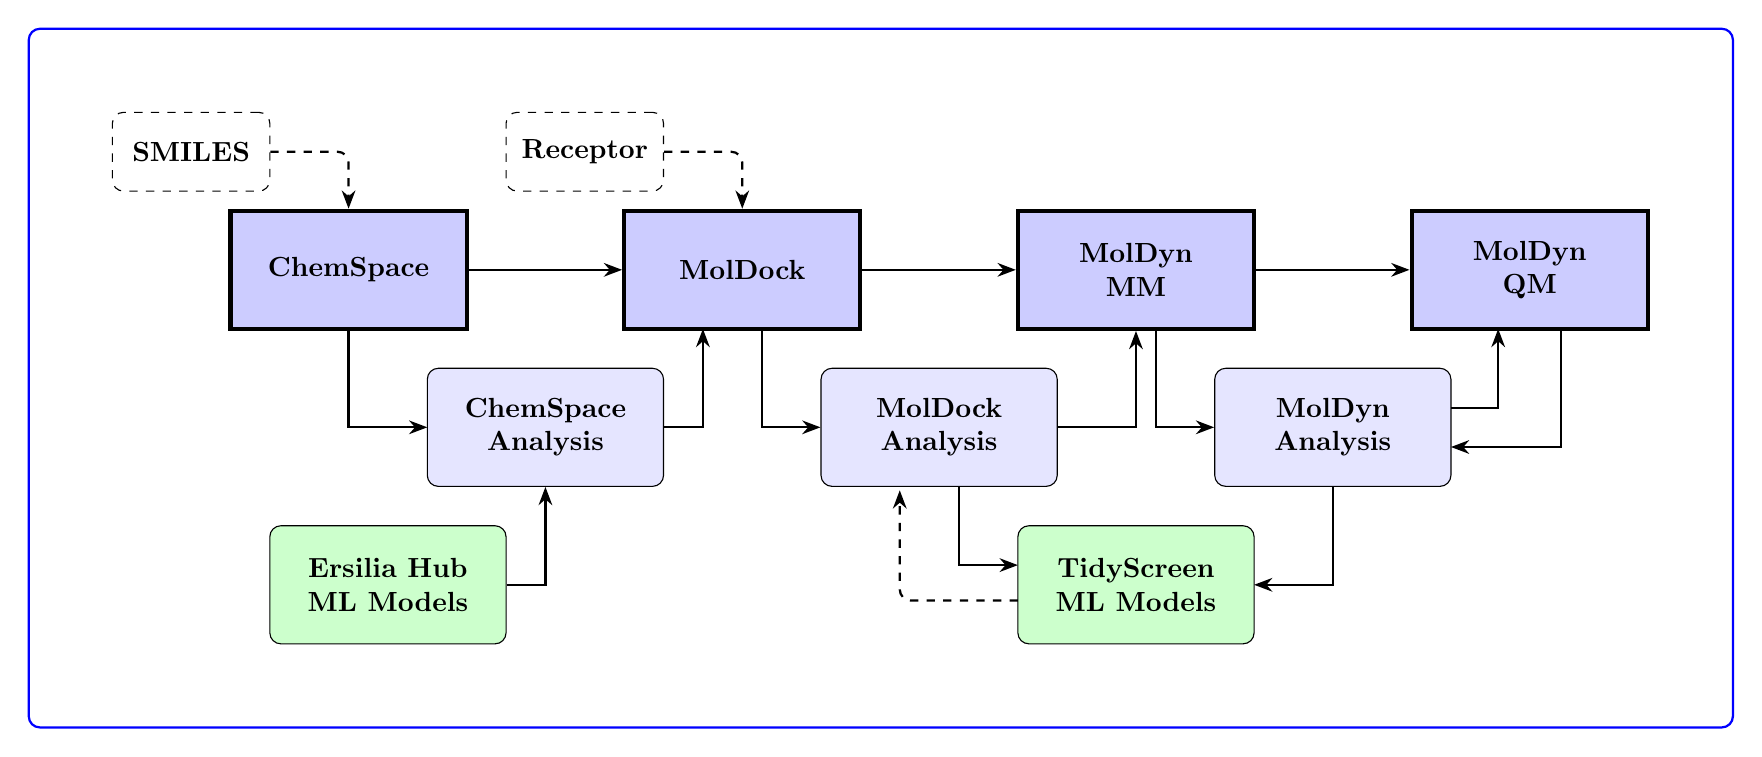
\begin{tikzpicture}[node distance=5cm, align=center, node/.style={draw, rectangle, minimum width=3.5cm, minimum height=2.5cm, rounded corners},
	boxaround/.style={draw=blue, thick, rounded corners, inner sep=30pt}]
	
	
		\node (chemspace) [process] {\textbf{ChemSpace}};
		
		\node (SMILES) at ($(chemspace)+(-2,1.5)$) [input] {\textbf{SMILES}};

		\node (moldock) [process, right of=chemspace] {\textbf{MolDock}};

		\node (receptor) at ($(moldock)+(-2,1.5)$) [input] {\textbf{Receptor}};
		
		\node (moldyn) [process, right of=moldock] {\textbf{MolDyn} \\ \textbf{MM}};
		
		\node (moldyn_QM) [process, right of=moldyn] {\textbf{MolDyn} \\ \textbf{QM}};
		
		\node (chemspace_analysis) at ($(chemspace)!0.5!(moldock)-(0,2)$) [process_analysis] {\textbf{ChemSpace} \\ \textbf{Analysis}};
		
		\node (Ersilia_Hub) at ($(chemspace_analysis)+(-2,-2)$) [plugin] {\textbf{Ersilia Hub} \\ \textbf{ML Models}};
		
		\node (moldock_analysis) at ($(moldock)!0.5!(moldyn)-(0,2)$) [process_analysis] {\textbf{MolDock} \\ \textbf{Analysis}};
		
		\node (moldyn_analysis) at ($(moldyn)!0.5!(moldyn_QM)-(0,2)$) [process_analysis] {\textbf{MolDyn} \\ \textbf{Analysis}};
	
		\node (TidyScreen_ML) at ($(moldock_analysis)!0.5!(moldyn_analysis)-(0,2)$) [plugin] {\textbf{TidyScreen} \\ \textbf{ML Models}};
	
	
		% The corresponding rows to connect nodes
		\draw [arrow_solid] (chemspace) --  (moldock);
		\draw [arrow_solid] (moldock) -- (moldyn);
		\draw [arrow_solid] (moldyn) -- (moldyn_QM);
		% -
		\draw [arrow_solid] (chemspace) |- +(1,-2.0) (chemspace_analysis);
		\draw [arrow_solid] (chemspace_analysis) -| +(2.0,1.25) (moldock) ;
		% -
		\draw [arrow_solid] (moldock) +(0.25,-0.75) |-  (moldock_analysis);
		\draw [arrow_solid] (moldock_analysis) -| (moldyn);
		% -
		\draw [arrow_solid] (moldyn) +(0.25,-0.75) |-  (moldyn_analysis);
		\draw [arrow_solid] (moldyn_analysis) +(1.5,0.25) -| +(2.1,1.25) (moldyn_QM);
		\draw [arrow_solid] (moldyn_QM) +(0.4,-0.75) |- +(-1,-2.25) (moldyn_analysis);
		
		% -
		\draw [arrow_solid] (moldock_analysis) +(0.25,-0.75) |- +(1.0,-1.75) (TidyScreen_ML);
		\draw [arrow_solid] (moldyn_analysis)  |-  +(-1.0,-2) (TidyScreen_ML);
		
		% Arrows corresponding to input nodes
		\draw [arrow_dashed] (SMILES) -| (chemspace);
		\draw [arrow_dashed] (receptor) -| (moldock);
		\draw [arrow_solid] (Ersilia_Hub) -| (chemspace_analysis);
		\draw [arrow_dashed] (TidyScreen_ML) +(-1.5,-0.20) -| +(-3.0,1.2) (moldock_analysis);
		
		
		% Rectangle around all nodes
		\node[boxaround, fit=(current bounding box)] {};
		
			
	\end{tikzpicture}
	
\end{document}



